\documentclass{article}

\usepackage{tikz}


\begin{document}
%   \maketitle
  \noindent
  \rule{\linewidth}{0.4pt}

  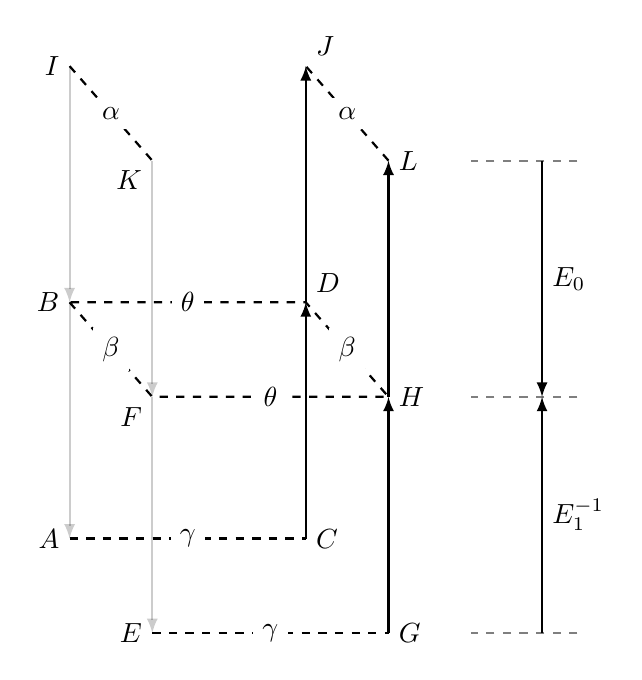
\begin{tikzpicture}[
    node distance = 5ex,
    scale = 3,
    thick,
    > = latex,
    % change the 
    z = {(0.35, -0.4)},
    edge/.style = {draw, thick, -, black},
    sinal/.style = {inner sep = 1pt, thin, opacity = 0.4,
      fill = blue, circle, text opacity = 1},
    mtx/.style = {
  %     matrix of math nodes,
      matrix of nodes,
      every node/.style = {
        anchor = base,
        text width = 2em,
        text height = 1em,
        align = center,
      }
    },
    ]

    \def\dist{0.1}
    \def\cube{
        % Vertices. (A,B,C), A x轴  B z轴  C y轴
        
        
        % \node[left] (v0) at (0,0,0) {$ A $};
        % note that command above can construct nodes and label them at the same time, 
        % but sometimes you don't need the text, 
        % so I just construct the coordinates and then label coordinates 
        \coordinate (v0) at (0, 0, 0)  ;
        \coordinate (v1) at (0, 1, 0)  ;
        \coordinate (v2) at (1, 0, 0)  ;
        \coordinate (v3) at (1, 1, 0)  ;
        \coordinate (v4) at (0, 0, 1)  ;
        \coordinate (v5) at (0, 1, 1)  ;
        \coordinate (v6) at (1, 0, 1)  ;
        \coordinate (v7) at (1, 1, 1)  ;
        \coordinate (v8) at (0, 2, 0)  ;
        \coordinate (v9) at (1, 2, 0)  ;
        \coordinate (v10) at (0, 2, 1) ;
        \coordinate (v11) at (1, 2, 1) ;
    }
    \begin{scope}[opacity=1] % opacity is the transparent 
        \cube{};
        % labeling verticals with text A B C at left\right\below\above\below left\below right\above left\above right
        \node[left] at (v0) {$ A $};
        \node[left] at (v1) {$ B $};
        \node[right] at (v2) {$ C $};
        \node[above right] at (v3) {$ D $};
        \node[left] at (v4) {$ E $};
        \node[below left] at (v5) {$ F $};
        \node[right] at (v6) {$ G $};
        \node[right] at (v7) {$ H $};
        \node[left] at (v8) {$ I $};
        \node[above right] at (v9) {$ J $};
        \node[below left] at (v10) {$ K $};
        \node[right] at (v11) {$ L $}; 
        % Edges with some differential: alpha gamma beta theta
        % arrow with direction from v1 to v0

        \draw[->] (v2) -- (v3);
        \draw[->] (v3) -- (v9);
        \draw[->] (v6) -- (v7);
        \draw[->] (v7) -- (v11);
        % dotted line from v1 to v2 and the middle of line labeled is gamma
        \draw[dashed] (v0) -- node[fill = white] {$ \gamma $} (v2) ;
        \draw[dashed] (v4) -- node[fill = white] {$ \gamma $} (v6);
        \draw[dashed] (v1) -- node[fill = white] {$ \beta $} (v5) -- node[fill = white] {$ \theta $} (v7) -- node[fill = white] {$ \beta $}(v3) -- node[fill = white] {$ \theta $} (v1);
        \draw[dashed] (v8) -- node[fill = white] {$ \alpha $}(v10);
        \draw[dashed] (v11) -- node[fill = white] {$ \alpha $}(v9);
    \end{scope}
        
    \begin{scope}[opacity=0.2]
        % the pics in this part are transparent 0.2, 
        % if not want this condition, delete the commands.
        \draw[<-] (v0) -- (v1);
        \draw[<-] (v1) -- (v8);
        \draw[<-] (v4) -- (v5);
        \draw[<-] (v5) -- (v10);
    \end{scope}
        
        % \foreach \i in {0, 1, ..., 11}{ \draw[fill = black] (v\i) circle (0.1pt); }
        % } % boomerang attack model
        
        \begin{scope}[]
            % 
            \coordinate (E0)  at (2, 0-0.4, 0);
            \coordinate (E0L) at (2-0.3, 0-0.4, 0);
            \coordinate (E0R) at (2+0.15, 0-0.4, 0);
            \coordinate (E1)  at (2, 1-0.4, 0);
            \coordinate (E1L) at (2-0.3, 1-0.4, 0);
            \coordinate (E1R) at (2+0.15, 1-0.4, 0);
            \coordinate (E2)  at (2, 2-0.4, 0);
            \coordinate (E2L) at (2-0.3, 2-0.4, 0);
            \coordinate (E2R) at (2+0.15, 2-0.4, 0);
            \draw[->] (E0) -- node[right] {$ E_1^{-1} $} (E1);
            \draw[->] (E2) -- node[right] {$ E_0 $} (E1);
            % dotted line with transparent 
            \draw[dashed,opacity=.5] (E0R) -- (E0) -- (E0L);
            \draw[dashed,opacity=.5] (E1R) -- (E1) -- (E1L);
            \draw[dashed,opacity=.5] (E2R) -- (E2) -- (E2L);
        % \foreach \i in {0, 1, ..., 11}{
        %   \node at (v\i) {\i}; 
        % }
      \end{scope}
    
    \end{tikzpicture}%
\end{document}